\documentclass[13pt]{article}
\usepackage[francais]{babel}
\usepackage[utf8]{inputenc}
\usepackage[T1]{fontenc}

\usepackage{verbatim}
\usepackage{amsthm}
\usepackage{amsmath,amssymb,amstext}
\usepackage{thmbox}
\usepackage{fancyhdr}
\usepackage{graphicx}
\usepackage{wrapfig}
\usepackage{url}


\newtheorem{bin}{  }
\newtheorem{format}{  }
\newtheorem{instr}
{ \textbf{Instructions actuellement prises en charges} }
\newtheorem{instrFutures}
{ \textbf{Instructions à venir} }

\newcommand{\cg}{[\kern-0.15em [}
\newcommand{\cd}{]\kern-0.15em ]}

\pagestyle{fancy}
\rhead{}

\title{Rapport du Projet de Système digital \no3}
\author{Belghiti Ismael, Desfontaines Damien, Geoffroy Guillaume, Maillard Kenji}
\date{\today}

\begin{document}
\renewcommand{\labelitemi}{$\triangleright$}

\maketitle
\tableofcontents

\section{Introduction}



\section{Le langage rock}

Le langage de description des circuits et un langage déclaratif basé sur la notion de bloc nommé \emph{rock}. Il y a trois types de blocs différents :
\begin{itemize}
\item Les blocs de base : xor, and, or, mux, not, ground, vdd et reg (déclarés dans Analysis/baseBlocks.ml)
\item Les blocs classiques pouvant être paramètrés par des entiers, prenant des fils en entrées et créant des fils en sorties, qui définissent leur corps à partir d'autres blocs.
\item Les périphériques ou blocs externes.
\end{itemize}

Il est compilé à l'aide du logiciel \emph{obsidian} dont l'organisation est montrée dans la figure 1. Les sections suivantes présentent les aspects spécifiques du langage et de sa compilation.

\begin{figure}[!h]
\centering
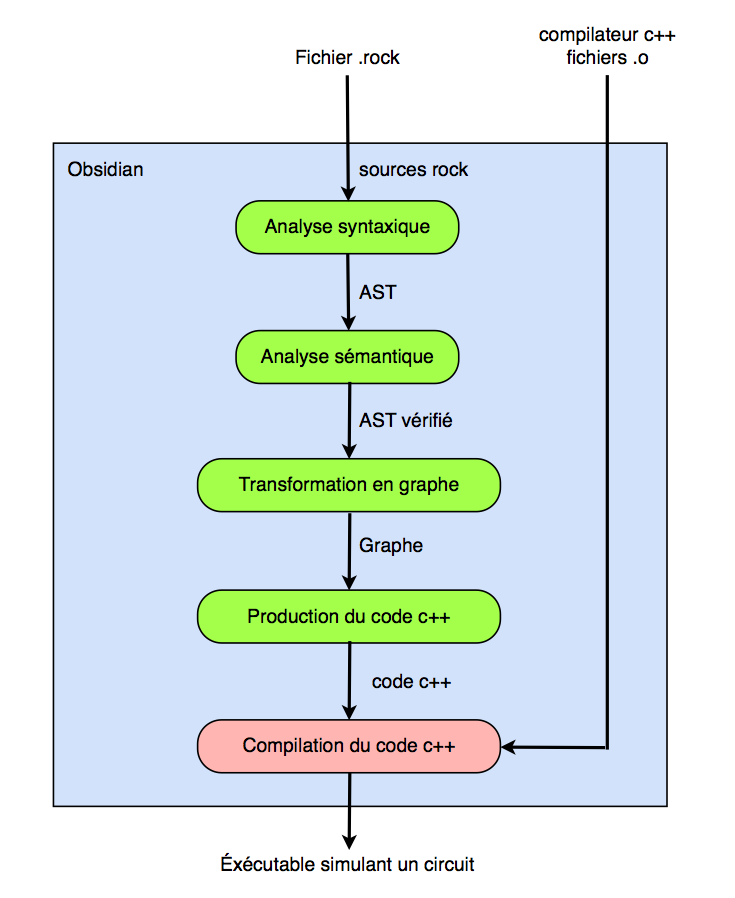
\includegraphics[width=14.7cm,height=17.96cm]{obsidian.png}
\caption{Architecture d'Obsidian}
\label{Architecture d'Obsidian}
\end{figure}

\subsection{Traitement lexical}
Le langage contient deux mots clés {\bf start} et {\bf device } ainsi que les
caractères {\bf <}, {\bf >}, {\bf (}, {\bf )}, {\bf $\to$}, {\bf ;}, {\bf :}, {\bf ,},
{\bf [}, {\bf ]}, {\bf \{}, {\bf \}}, {\bf .}, {\bf ..}, {\bf +}, {\bf -}, {\bf *}, {\bf /},
{\bf \%}, {\bf \^{}}, {\bf @}. 

Les identifiants sont de l'une des deux formes suivantes :
\begin{description}
\item[NomBloc : ] un identifiant commençant par une majuscule, il sert à
  identifier les blocs et les variables de blocs.
\item[NomFil : ] identifiant commençant par une minuscule, il sert à identifier
  les noms de fils et de variables entières.
\end{description}

L'opération d'analyse lexicale se charge aussi d'effacer les commentaires qui
sont soit de la forme \og $(*$\fg{} \og $*)$\fg{} pour les commentaires
multi-lignes, soit de la forme \og \#\fg{} pour les commentaires sur une seule ligne.

\subsection{Syntaxe du langage}
Le langage suit la grammaire suivante :\newline\newline
\begin{tabular}{ r c l }
  fichier &$::=$&\: instruction* BlocEntrée instruction*\\ [1.5ex]
  BlocEntrée &$::=$&\: {\bf start} NomBloc $<$ ConstanteEntière, ... ,
  ConstanteEntière  $>$\\ [1.5ex]
  instruction &$::=$&\: BlocDéfinition\\
  &&| PériphériqueDéfinition \\ [1.5ex]
  BlocDéfinition &$::=$&\: NomBloc Paramètres? Arguments? Instance* $\to$
  Sorties $;$\\ [1.5ex]
  PériphériqueDéfinition &$::=$&\: {\bf device} NomBloc Paramètres\\ [1.5ex]
  Paramètres &$::=$&\: $<$ Motif, ... , Motif $>$\\ [1.5ex]
  Motif &$::=$&\: $a*n+k+b$     \\ 
  &&| $a*n+b$  \\ 
  &&| $b$ \\ 
  \multicolumn{3}{c}{(avec $a$, $b$ des constantes entières, $a
    \neq 1$ et $n$, $k$ des identifiants de variables)} \\ [1.5ex]
  Arguments &$::=$&\: $($ DeclarationFil, ... , DeclarationFil $)$ \\ [1.5ex]
  DeclarationFil  &$::=$&\: NomFil \\
  &&| NomFil $[$ ConstanteEntière $]$ \\ [1.5ex]
 
  Instance &$::=$&\: NomBloc NomVariableBloc $($ Fil, ... , Fil $)$ \\ [1.5ex]
  Fil &$::=$&\: NomFil\\
  &&| NomVariableBloc {\bf .} NomFil\\
  &&| NomFil $[$ ConstanteEntière $]$\\
  &&| NomFil $[$ ConstanteEntière {\bf..} ConstanteEntière $]$\\
  &&| {\bf \$} $(0|1)+$ \\
  &&| $\mathbf{\{}$ Fil, ... , Fil $\mathbf{\}}$\\ [1.5ex]
  Sorties&$::=$&\: DeclarationFil : Fil, ... , DeclarationFil : Fil
\end{tabular}


\subsection{Les entiers} 
Les entiers sont présents en rock à deux niveaux : 
\begin{itemize}
\item Dans les paramètres pour permettre la récursion.
\item Dans les fils pour préciser leur taille.
\end{itemize}
\text{}\\

On peut les écrires tout aussi bien en hexadécimal (préfixe \og $0x$\fg{} ou \og $0X$\fg{}), en
octal (préfixe \og $0o$\fg{} ou \og $0O$\fg{}), en binaire (préfixe \og $0b$ \og
ou \og $0B$\fg{}) ou en décimal (sans préfixe).
Ils supportent les opérations suivantes :
\begin{itemize}
\item $+$ l'addition
\item $-$ la soustraction
\item $*$ le produit
\item $/$ le quotient dans la division euclidienne
\item $\%$ le reste dans la division euclidienne
\item \^{} l'exponentiation
\end{itemize}


\section{Concepts clés du langage}

Le langage rock est muni de plusieurs concepts qui en font un outil maniable,
utile, voir efficace : il s'agit de la récursion, des périphériques et des enables.

\subsection{Motifs et récursion}
Le langage ne dispose pas des opérations classiques comme \texttt{for},
\texttt{while} ou \texttt{if} pour manipuler le flôt d'éxécution. Il est par
contre doté d'un système puissant de récursion et de reconnaissance de motifs.
Il y a deux types de motifs :
\begin{itemize}
\item les motifs constants qui n'acceptent que la valeur de leur constante. 
\item les motifs de la forme $ a*n + b $, avec $a$, $b$ constants et $n$
  variable, qui acceptent les entiers $p$  tels que $p \equiv b\
  \text{mod}\ a$ et on a alors $n = \frac{p - b}{a}$.
\item les motifs de la forme $ a*n + k + b $, avec $a \neq 1 $, $b$ constants et
  $n$ variable, qui acceptent tous les entiers $p$ en posant $k \equiv  p - b\
  \text{mod}\ a$, $0 \leq k < a$ et $n = \frac{p - b - k}{a}$.
\end{itemize}
\text{}\\
Étant donné un entier $p$ et une liste ordonnée de motifs $(m_i)_i$, les motifs
fonctionnent selon le principe suivant : 
\begin{itemize}
\item l'entier est testé sur le $i^{e}$motif.
\item s'il est accepté, les variables correspondant au motif sont assignés si
  nécessaire.
\item s'il est rejeté, on passe au motif $i+1$.
\item si aucun motif ne convient, le compilateur lève une erreur.
\end{itemize}
\text{}\\
La récursion devient alors assez immédiate :
\begin{itemize}
\item On peut itérer sur tous les entiers avec les motifs $<n+1>$ et $<0>$.
\item Ou seulement sur les puissances de deux avec les motifs $<2*n>$ et $<1>$.
\item Ou travailler sur des congruences modulo 3 avec les motifs $<3*n>$, $<3*n +
  1>$ et $<3*n + 2>$.
\end{itemize}
\text{}\\
Un point important limite cependant l'expressivité de cet outil : à l'intérieur
d'un bloc ayant comme paramètres les entiers $(n_i)_i$, seuls des blocs avec
des paramètres plus petit (au sens de l'odre sur $\mathfrak{N}$) peuvent être
instancier. Ce critère permet notamment d'assurer la terminaison des calculs et
surtout la terminaison de la compilation en assurant qu'il n'y a pas de chaine
infini de blocs.

\subsection{Les périphériques}


Les périphériques sont un moyen de définir de nouvelles portes en plus des
portes base. On peut les utiliser pour simuler des mémoires, ou des
périphériques d'entrée/sortie.

Tous les périphériques ont la même interface (les mêmes fils d'entrée et
les mêmes fils de sortie) :
\begin{itemize}
\item Entrée :
\text{}\\
\text{}\\
  \begin{tabular}{ | c | c | }
    \hline
    Address &  32 bits \\
    \hline
    Data & 32 bits \\
    \hline
    Write mode & 1 bit\\
    \hline
    Byte enables &  4 bits\\
    \hline
    Enable interrupt & 1 bit\\
    \hline
    Interrupt processed & 1 bit\\
    \hline
  \end{tabular}
\text{}\\
\item Sortie :
\text{}\\
\text{}\\
 \begin{tabular}{ | c | c | }
    \hline
    Data &  32 bits \\
    \hline
    Interrupt request & 1 bit \\
    \hline
  \end{tabular}
\end{itemize}

Les périphériques peuvent contenir du code arbitraire, et peuvent donc a
priori gérer leurs entrées et sorties de n'importe quelle
manière. Cependant, ils sont faits pour simuler des périphériques mappés en
mémoire : Les entrées \texttt{Address}, \texttt{Data} et \texttt{Write mode} et
la sortie \texttt{Data} 
fonctionnent comme leur nom l'indique (l'entrée \texttt{Data} contient les données
à écrire si \texttt{Write mode} $=  1$, la sortie \texttt{Data} contient les données lues).
L'entrée \texttt{Byte enables} indique quels octets il faut prendre en compte :
\begin{itemize}
\item   Si à l'adresse $0$ se trouve la suite d'octets $11\ 22\ 33\ 44$, et si l'on
    essaye de lire à l'adresse $0$ avec \texttt{Byte enables} = $\$1010$, la valeur lue
    correspondra à la suite d'octets $11\ 00\ 33\ 00$.

\item  Si à l'adresse $0$ se trouve la suite d'octets $11\ 22\ 33\ 44$, et si l'on
    essaye d'écrire $55\ 66\ 77\ 88$ à l'adresse $0$ avec \texttt{Byte enables} $= \$1010$,
    on trouvera à l'adresse $0$ la suite d'octets $55\ 22\ 77\ 44$.
\end{itemize}

Les périphériques sont pensés comme des registres, c'est-à-dire que si l'on
écrit l'adresse où l'on veut lire au cycle t, on pourra lire le résultat au
cycle t+1. A posteriori, il aurait été plus pratique de donner le choix
entre les deux modes de fonctionnement (lecture instantannée et lecture
retardée d'un cycle), car lorsqu'un périphérique n'est pas utilisé pour
couper une boucle combianatoire, on perd simplement un cycle à attendre.

On déclare les types de périphériques de la façon suivante :

\begin{verbatim}
  device Memory<size>
\end{verbatim}

Puis, le type de périphérique peut être instancié comme n'importe quel
autre type de bloc, par exemple, le circuit suivant :
\begin{verbatim}
  Start
      Memory<5> Ram($0000...0000, $0000...0000, $1111, $0, $0)
      -> out[32] : Ram.dtata;

  start Start
\end{verbatim}
Est constitué d'une mémoire sur $2^5 = 32$ octets, et sa sortie correspond au
mot de $32$ bits contenu à l'adresse $0$ dans la mémoire. Si la mémoire est
prévue pour initialiser tous ses octets à $0$, la sortie de ce circuit sera :

\begin{verbatim}
  00000000000000000000000000000000
  00000000000000000000000000000000
  00000000000000000000000000000000
  00000000000000000000000000000000
  ...
\end{verbatim}

Et le circuit suivant :

\begin{verbatim}
  Start
      Memory<5> Ram($0000...0000, $1111...1111, $1100, $1, $0)
      -> out[32] : Ram.dtata;

  start Start
\end{verbatim}

Aura pour sortie :

\begin{verbatim}
  00000000000000000000000000000000
  11111111111111110000000000000000
  11111111111111110000000000000000
  11111111111111110000000000000000
  ...
\end{verbatim}

On définit les types périphériques de la manière suivante :
Chaque type de périphérique est défini par une classe C++, qui doit
descendre de la classe device :
\begin{verbatim}
  class device
  {
  public :
    virtual ~device();
    virtual unsigned int cycle (unsigned int address, unsigned int data,
                                char byte_enables, bool write_enable,
                                bool interrupt_enable, bool iack, char *
                                irq)=0;
  };
\end{verbatim}
Chaque périhérique doit également fournir une méthode statique \texttt{make}, qui
construit un objet de cette classe et renvoie un pointeur vers cet objet,
upcasté en \emph{device*}. Cette méthode prend un argument (de type \emph{int}) par
paramètre du périphérique. Par exemple, pour le périphérique \texttt{Memory}, la
méthode \texttt{make} a le prototype suivant :

\begin{verbatim}
  device * make (int size)
\end{verbatim}

Pour chaque périphérique du circuit, sa méthode "cycle" est appelée à
chaque cycle, avec comme arguments les valeurs lues dans les fils d'entrée.


\subsection{Les enables}

Les enables permettent de redéfinir localement l'horloge du circuit :
le circuit suivant :
\begin{verbatim}
  Count_mod_2
      Not N(R.o)
      Reg R(N.o)
      -> o : R.o ;

  Start
      Count_mod_2 C1
      Count_mod_2 @ C1.o C2
      -> o : C2.o ;

  start Start
\end{verbatim}

Contient deux compteurs modulo 2 : C1 et C2, mais à l'intérieur du second,
l'horloge est localement redéfinie, de sorte que le second compteur n'est
actif qu'au cycles où la sortie du premier vaut 1, c'est-à-dire un cycle
sur deux. La sortie du circuit est donc :

\begin{verbatim}
  0
  0
  1
  1
  0
  0
  1
  1
  ...
\end{verbatim}
Lorsqu'une porte n'est pas active, le code C++ correspondant n'est
simplement pas exécuté : La sortie de la porte garde sa valeur du cycle
précédent, et s'il s'agit d'un registre, son contenu n'est pas
modifié. Dans le cas d'un périphérique, sa méthode "cycle" n'est pas
appelée.


Si on redéfinit l'horloge d'un bloc, on redéfinit l'horloge de toutes les
portes et de tous les blocs qu'il contient. Si ce bloc lui-même redéfinit
l'horloge de l'un de ses composants, celui-ci ne sera actif que lorsque son
bloc parent l'est et que son bloc parent l'active. Par exemple, on peut
utiliser les enables pour programmer un compteur modulo $2^n$ : Le bloc
suivant :
\begin{verbatim}
  Count<1>
      Reg M(N.o)
      Not N(M.o)
      -> out : M.o,
         carry : M.o;

  Count<n>
      Count<1> Low
      Count<n-1> @ Low.carry High
      And A(Low.carry, High.carry)
      -> out[n] : {Low.out, High.out},
         carry : A.o;

  Start<n>
      Count<n> C
      -> out[n] : C.out;

  start Start<3>
\end{verbatim}
A pour sortie :
\begin{verbatim}
  000
  100
  010
  110
  001
  101
  011
  111
  000
  100
  010
  ...
\end{verbatim}

L'intérêt majeur des enables est qu'ils permettent de gagner du temps en
n'exécutant que les parties du circuit qui sont utiles au cycle en cours
(en plus de rendre certains codes plus simples, comme celui du compteur
modulo $2^n$). Par exemple, grâce aux enables, on peut définir un bloc
\texttt{Ram} de manière (à peu près) efficace :
\begin{verbatim}
  Mux_scalar <1> (selector, input0[1], input1[1])
      Mux M(selector, input0, input1)
      -> o : M.o;

  Mux_scalar <n> (selector, input0[n], input1[n])
      Mux_scalar<n-1> Low(selector, input0[0..n-2], input1[0..n-2])
      Mux High(selector, input0[n-1], input1[n-1])
      -> o[n] : {Low.o, High.o};

  Ram <0,1> (data[1], write)
      Mux M(write, R.o, data[0])
      Reg R(M.o)
      -> data[1] : R.o;

  Ram <0,d> (data[d], write)
      Ram<0,d-1> Low(data[0..d-2], write)
      Ram<0,1> High(data[d-1], write)
      -> data[d] : {Low.data, High.data};

  Ram <1,d> (address[1], data[d], write)
      Not N(address[0])
      Ram<0,d> @ address[0] Low(data, write)
      Ram<0,d> @ N.o        High(data, write)
      Mux_scalar<d> M(address, Low.data, High.data)
      -> data[d] : M.o;

  Ram <a,d> (address[a], data[d], write)
      Not N(address[a-1])
      Ram<a-1,d> @ N.o          Low(address[0..a-2], data, write)
      Ram<a-1,d> @ address[a-1] High(address[0..a-2], data, write)
      Mux_scalar<d> M(address[a-1], Low.data, High.data)
      -> data[d] : M.o;
\end{verbatim}
Ainsi, pour une mémoire de $2^a$ mots de $d$ bits, le temps de calcul pour un
cycle est en $O(a*d)$, au lieu du $O(2^a * d)$ que l'on aurait eu sans enables.


\subsection{Exemples de codes et de blocs classiques}
Voici quelques exemples de blocs que l'on peut définir avec ce langage :

\begin{verbatim}
### Manipulations de fils épais ###
\end{verbatim}

On peut effectuer diverses opérations sur les fils épais, par exemple le
renversement :

\begin{verbatim}
  Rev<1> (in[1])
      -> out[1] : in[0];

  Rev<n> (in[n])
      Rev<n-1> High(in[1..n-1])
      -> out[n] : {High.out, in[0]};
\end{verbatim}

On peut aussi étendre les opérations à des fils épais, bit-à-bit :

\begin{verbatim}
  And_vect<1> (a[1],b[1])
      And A(a[0],b[0])
      -> o : A.o;

  And_vect<n> (a[n],b[n])
      And Low(a[0],b[0])
      And_vect<n-1> High(a[1..n-1],b[1..n-1])
      -> o[n] : {Low.o, High.o};
\end{verbatim}

Ou à la manière d'un produit par un scalaire :

\begin{verbatim}
  And_scalar<1> (a,b[1])
      And A(a,b[0])
      -> o : A.o;

  And_scalar<n> (a,b[n])
      And Low(a,b[0])
      And_scalar<n-1> High(a,b[1..n-1])
      -> o[n] : {Low.o, High.o};
\end{verbatim}

Ou encore à la manière d'un fold :

\begin{verbatim}
  And_fold <1> (a[1])
      -> o : a;

  And_fold <n> (a[n])
      And_fold<n-1> Tail(a[0..n-2])
      And Head(a[n-1], Tail.o)
      -> o : Head.o;
\end{verbatim}
\begin{verbatim}
### Constantes ###
\end{verbatim}
On peut associer automatiquement à un entier n un fil épais représentant n
sur p bits :
\begin{verbatim}
  Bin<0,1>
      -> o : $0;
  Bin<1,1>
      -> o : $1;

  Bin<2*n,p>
      Bin<n,p-1> High
      -> o[p] : {$0, High.o};
  Bin<2*n+1,p>
      Bin<n,p-1> High
      -> o[p] : {$1, High.o};
\end{verbatim}
\begin{verbatim}
### Compteurs modulo n ###
\end{verbatim}
On peut tout d'abord définir un compteur modulo $2^{n}$ :
\begin{verbatim}
  Count<1> (enable)
      Reg R(X.o)
      Xor X(R.o,enable)
      And A(R.o,enable)
      -> out : R.o,
         carry : A.o;

  Count<n> (enable)
      Count<n-1> Low(enable)
      Count<1> High(Low.carry)
      -> out[n] : {Low.out, High.out},
         carry : High.carry;
\end{verbatim}
On peut aussi ajouter un argument "reset" au compteur :
\begin{verbatim}
  Count_reset<1> (e, r)
      Reg Mem(New_value.o)

      Not Not_reset (r)
      And New_value (Result.o, Not_reset.o)

      Xor Result(Mem.o,e)
      And Carry(Mem.o,e)
      -> o : Mem.o, c : Carry.o;

  Count_reset<n> (e, r)
      Count_reset<n-1> L(e, r)
      Count_reset<1> H(L.c, r)
      -> o[n] : {L.o, H.o}, c : H.c;
\end{verbatim}
Et à partir de là, on peut définir un compteur modulo n sur p bits :

Il faut d'abord définir une opération "égalité" sur des fils épais :
\begin{verbatim}
  Xor_vect<1> (a[1],b[1])
      Xor X(a[0],b[0])
      -> o : X.o;
  Xor_vect<n> (a[n],b[n])
      Xor Low(a[0],b[0])
      Xor_vect<n-1> High(a[1..n-1],b[1..n-1])
      -> o[n] : {Low.o, High.o};

  Not_vect<1> (a[1])
      Not N(a[0])
      -> o : N.o;
  Not_vect<n> (a[n])
      Not Low(a[0])
      Not_vect<n-1> High(a[1..n-1])
      -> o[n] : {Low.o, High.o};

  Is_equal<n> (a[n],b[n])
      Xor_vect<n> Not_equal(a,b)
      Not_vect<n> Equal(Not_equal.o)
      And_fold<n> All_equal(Equal.o)
      -> o : All_equal.o;
\end{verbatim}

Et le compteur :
\begin{verbatim}
  Counter<n,p> (e)
      Count_reset<p> C(e, Reset.o)
      Bin<n-1,p> Mod
      Is_equal<p> Reset(C.o,Mod.o)
      -> o[p] : C.o;
\end{verbatim}


\section{Spécificités techniques de l'implémentation d'Obsidian}

ocamllex et menhir pour lexing et parsing

sur -> analyse sémantique lourde mais efficace
    static bound checking
    vérification du caractère bien fondé des récursions

union-find pour détruire le graphe en ast

compilation vers du c++ pour les performances

\section{Le microprocesseur}

L'architecture du microprocesseur a été modifiée depuis le dernier rapport.
Nous utilisons maintenant des périphériques pour gérer la mémoire, les registres
et le programme. Le nombre d'instructions supportées a été considérablement 
augmenté. D'une architecture à trois cycles par instruction, nous sommes passés
à une architecture à 4 cycles par instruction permettant une grande sécurité des
échange du controleur, les périphiques assurant parallèlement une protection contre
les boucles combinatoires.

\subsection{L'ALU}

L’ALU que nous avons réalisé prend en entrée deux entiers sur
32 bits ainsi qu’un code sur 4 bits décrivant l’opération à effectuer. Il renvoie
alors un résultat sur 32 bits. Il s’agit d’un bloc purement combinatoire.\\

Notre ALU supporte 16 opérations :

\begin{enumerate}
\item ET, OU, XOR, NAND, NOR pour les opérations logiques binaires
\item $+$,$-$,$x$,$=$,$\neq$,$<$,$>$,$\leq$,$\geq$ pour les opérations arithmétiques
\item Une opération renvoyant le premier opérande (utile pour les opérations de shifts)
\item Une opération de concaténation 16 bit-16 bit (utile pour le \textit{lui})
\end{enumerate}  

D'autres opérations ont été implémentées, notamment les différentes formes de shift 
(dans les deux sens, en version classique ou arithmétique) cependant seule l'opération
de shift classique vers la droite est utilisé par le reste du microprocesseur (il
est utilisé avec le shift\_amount du R-format ).

\textbf{Fonctionnement:} Chaque opération de l’ALU est codée séparément.
Puis, à la lecture de deux entiers, toutes les opérations possibles sont exécutées
simultanément, et un filtre sélectionne le résultat voulu. Tout fonctionne en un
seul cycle, et les circuits correspondant aux diverses opérations ont tous été
codés récursivement.

\subsection{Registres, Instruction Memory et Data Memory } 

Le gestionnaire de registres contient 32 registres de 32 bits chacun.
Il s'agit d'un périphérique de type mémoire. Il est possible de faire plusieurs
lectures simultanées (un nombre arbitrairement grand) en utilisant des périphériques
lecteurs auxiliaires. Dans notre cadre, on accède à au plus à deux registres à la fois, un seul 
périphérique auxiliaire de lecture suffit donc. \\

Le bloc d'instructions est également un périphérique. Chaque instruction est stockée
sur 32 bits. Nous suivons les différents format MIPS (R-format, I-format, J-format) mais
nous traitons à part certaines opérations de ces formats pour faciliter 
et mieux diviser le travail du 
controleur, comme nous le verrons dans la section Instructions.

Enfin, la Data Memory peut prendre deux formes, selon que l'on est en mode ''classique"
ou en mode ``horloge'' avec un affichage 7-segments. 

\subsection{Controleur}

Le bloc de contrôle, présent dans notre projet sous le nom de ``Controleur''
a dans notre projet non seulement le rôle du bloc ``Control'' de l’architecture
standart MIPS mais c’est aussi lui qui s’occupe de la synchronisation entre les
différents cycles parcourus pour une instruction donnée (Tous les autres blocs
sont donc positionnés en étoile par rapport à lui). Cette synchronisation est
obtenue et sécurisée par l’utilisation de filtres temporels gérant les trafics d’in-
formations entre les différents blocs. Toutes les instructions sont executées sur
quatre cycles.

Ce controleur agit différemment selon le format de l’instruction à effectuer,
il contient donc plusieurs décodeurs. Nous avons 3 decodeurs correspondant
aux formats MIPS habituels : un pour le R-format, un pour le I-format, 
un pour le J-format. Mais nous avons préféré traiter certains types d'instructions
à part, car elles correspondent à des échanges spécifiques entre les différents blocs 
du microprocesseur. Ainsi, nous avons 4 decodeurs plus spécifiques : un pour les écritures en 
mémoire (sb et sw), un pour les lectures mémoires (lb et lw), un pour les branch et enfin
un pour jr. 

Ces decodeurs sont executés en parallèle mais le controleur agit comme un filtre
et ne laisse transparaitre que les actions du decodeur correspondant à l'instruction en cours.
Ce filtrage s'effectue selon la valeur de l'opcode de l'opération.

\subsection{Instructions}

Les instructions suivent un codage relativement classique.
Décrivons les intervalles de bits de chacun des types d'instructions :


\subsubsection{R-format}

Ce format intervient par exemple dans les opérations 
comme add, sub, mul, and, ...

\begin{format}[codage du R-format]
  \begin{itemize}
  \item 0..5 : les 6 bits de l'opcode
  \item 6..10 : adresse rs (opérande 1)
  \item 11..15 : adresse rt (opérande 2)
  \item 16..20 : adresse rd (résultat)
  \item 21..25 : shift\_amount
  \item 26..31 : funct code
  \end{itemize}
\end{format}

Les 6 bits de l'opcode sont toujours nuls ainsi que les deux
derniers chiffres du funct code. Les quatre premiers bits du
funct code correspondent, eux, au code de l'opération concernée
(c'est ce code qui est transmis à l'ALU). Enfin le shift\_amount 
correspond à la valeur de décalage d'un shift vers la droite 
(c'est-à-dire à une division par une puissance de 2).

\subsubsection{I-format}

Le I-format correspond aux instructions du type addi, subi, andi...

\begin{format}[codage du I-format]
  \begin{itemize}
  \item 0..5 : les 6 bits de l'opcode
  \item 6..10 : adresse rs (opérande 1)
  \item 11..15 : adresse rt (resulat)
  \item 16..31 : valeur immédiate (opérande 2)
  \end{itemize}
\end{format}

Les deux derniers bits de l'opcode sont toujours deux 1.
Les quatre premiers bits de l'opcode correspondent, eux, au code
de l'opération de l'ALU. La valeur immédiate est étendue sur 
32 bits par la droite en répétant son dernier bit 
(afin de gérer les nombres négatifs).

\subsubsection{J-format}

On définit ici un format pour la seule instruction Jump.

\begin{format}[codage du J-format]
  \begin{itemize}
  \item 0..5 : les 6 bits de l'opcode
  \item 6..31 : adresse de la destination sur 26 bits
  \end{itemize}
\end{format}

L'opcode est toujours 111101. 

\subsubsection{Branch-format}

Le Branch-format regroupe les différentes instructions
de type branch comme beq, bne, bgt, ble...

\begin{format}[codage du Branch-format]
  \begin{itemize}
  \item 0..5 : les 6 bits de l'opcode
  \item 6..10 : adresse rs (opérande 1)
  \item 11..15 : adresse rt (opérande 2)
  \item 16..31 : adresse relative en cas de branch
  \end{itemize}
\end{format}

Les deux derniers bits de l'opcode sont toujours 10 tandis que
les quatres premiers bits correspondent au code de l'opération de 
l'ALU associée (par exemple le code de l'égalité pour un beq).
L'adresse relative est définie par rapport à l'adresse qui suit 
l'instruction branch.


\subsubsection{JR-format}

L'instruction Jump Register bénéficie d'un format à part.

\begin{format}[codage du JR-format]
  \begin{itemize}
  \item 0..5 : les 6 bits de l'opcode
  \item 6..10 : adresse du registre
  \item 11..31 : bits inutilisés
  \end{itemize}
\end{format}

L'opcode est toujours 000001.


\subsubsection{Format de lecture mémoire}

Ce format correspond aux instructions lw et lb.

\begin{format}[codage du format de lecture]
  \begin{itemize}
  \item 0..5 : les 6 bits de l'opcode
  \item 6..10 : adresse rs (registre contenant l'adresse de base) 
  \item 11..15 : adresse rt (resulat)
  \item 16..31 : valeur immédiate de décalage
  \end{itemize}
\end{format}

L'opcode est soit 110001 pour lw, soit 100001 pour lb. En pratique, 
le deuxième bit de l'opcode est repassé en argument au byte\_enable
de la mémoire (pour spécifier la plage de lecture).
 
\subsubsection{Format de l'écriture mémoire}

Ce format correspond aux instructions sw et sb.

\begin{format}[codage du format d'écriture]
  \begin{itemize}
  \item 0..5 : les 6 bits de l'opcode
  \item 6..10 : adresse rs (registre contenant l'adresse de base) 
  \item 11..15 : adresse rt (registre à stocker)
  \item 16..31 : valeur immédiate de décalage
  \end{itemize}
\end{format}

L'opcode est soit 110101 pour lw, soit 100101 pour lb. Ici aussi, 
le deuxième bit de l'opcode est repassé en argument au byte\_enable
de la mémoire (pour spécifier la plage d'écriture).


\section{L'assembleur}

\section{L'horloge}

Le fichier horloge.s est le fichier assembleur qui code l'horloge (d'où son nom,
incroyable, n'est-il pas ?). Son fonctionnement est le suivant :

\begin{enumerate}
\item Il va chercher le timestamp courant dans l'adresse mémoire ayant comme label
   \emph{timestamp}. Le format est celui du timestamp UNIX standard, accessible (par
   exemple avec la commande \texttt{date +\%s}. Pour mémoire, il s'agit du nombre de
   secondes écoulées depuis le $1^{\text{er}}$ janvier $1970$ à $00:00:00$.\\
\item Il transforme ce nombre de secondes en nombre de jours en faisant une simple
   division (codée plus loin, car indisponible dans notre microprocesseur, à
   partir d'une multiplication, elle aussi recodée avec des additions - de façon
   logarithmique bien sûr).\\
\item En prenant le reste de la division précédente, et par divisions successives,
   il est très facile d'obtenir l'heure de la journée. Ce calcul est donc
   effectué puis affiché dans l'afficheur $7$ segments (la méthode pour cela est
   décrite à part).\\
\item Puis, on doit calculer la date. Et là, c'est nettement plus technique. Il
   faut commencer par corriger les décalages dûs aux années bissextiles. Deux
   approches sont essentiellement possibles : considérer qu'une année "normale"
   est une année de $365$ jours, et prévoir un cas précis pour certains timestamps
   correspondant aux quelques $29$ févriers ; ou bien considérer qu'une année
   "normale" fait $366$ jours et se contenter de modifier en dur le timestamp en
   ajoutant l'équivalent d'un jour chaque $28$ février à $23:59:59$ d'une année non
   bissextile. C'est cette deuxième option qui a été choisie.\\
\item On calcule donc le nombre de jours à ajouter, par paquets de $4$ ans (on
   rajoute $72$ heures à chaque fois) et en corrigeant en bout de course. On fait
   un cas particulier pour l'an $2000$ (année non bissextile, comme tous les $400$
   ans - heureusement, le timestamp UNIX s'arrête en $2038$, on est donc pas tenus
   de prévoir les autres cas), et finalement on obtient un nombre de jours
   "artificiels" mais qui permet de traiter tous les cas d'un seul coup.
\item On calcule le mois et le jour en faisant $12$ cas, faute de méthode plus simple
   pour s'adapter aux durées variables des différents mois. Pour le mois de
   février, un des avantages est que l'on peut toujours considérer qu'il dure $29$
   jours - la modification précédente du timestamp garantit que l'on ne peut pas
   tomber dans le cas "$29$ février" si on n'est pas une année bissextile.
\item On affiche enfin la date, et on revient au début pour récupérer le nouveau
   timestamp et recommencer. "Un programme n'est pas fait pour être arrêté."
\end{enumerate}

Pour afficher la date, il faut d'abord transformer un nombre sur un octet en
format "afficheur $7$ segments" (où chaque bit représente l'état, allumé ou
éteint, d'un des $7$ segments). La traduction est codée en dur, dans deux tables
(selon si les nombres considérés ont deux (cas le plus courant) ou quatre
chiffres (pour les années par exemple)) nommées \texttt{two\_digits\_to\_segments} et
\texttt{year\_to\_segments}, et il suffit de chercher au bon endroit de ces tables (au
début pour $00$, dans les deux cases suivantes pour $01$, etc.) pour avoir
le renseignement voulu. Puis, on stocke le résultat en dur dans des cases
mémoires reliées directement à l'afficheur $7$ segments.

\begin{figure}[!h]
\centering
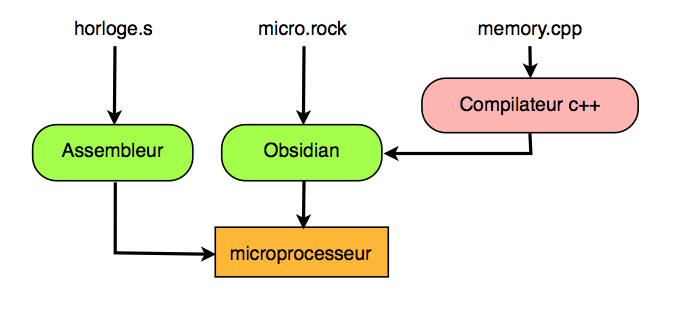
\includegraphics[width=13.5cm,height=6.2cm]{exec.png}
\caption{Architecture d'Obsidian}
\label{Architecture d'Obsidian}
\end{figure}

\end{document}
